%!TEX root = Report.tex

\subsection{Tracking}
\label{tracking}
As mentioned in the project proposal the project was divided into three parts. The first part of the project was to be able to track termites. Since African termites are hard to come by and transport we settled for giant ants (Camponotus Ligniperdus), which are the largest ants found in Denmark \cite{fogn}, instead. While these are not as big as the termites, they behave in a similar way and the solution should be easily adaptable to termites. In the first part we started by implementing the tracking on a video. We received a video from Harvard University of a single ant capturing the entire petri dish with a white background. The ant itself was painted red and green. This was the simplest setup we could think of and acted as a good starting point. By recommendation we decided to use the OpenCV \cite{opencv} framework. We will return to this framework in Section \ref{framework}.\\

This chapter is divided into three subparts. First we will different image processesing techniques, and their use. Following this we will discuss the OpenCV framework, and finish off describing the implemented solution and design choices.

% Gå ud fra at dette afsnit ikke har noget video input fra et kamera. Integration med kameraet kommer senere.
% 
% Teori først - hvilken slags image manipulation har vi brugt? hvad var alternativerne?
% Så framework - vi bruger OpenCV, why? hvad giver det os? hvad er drawbacks?
% så implementation - Hvad har vi implementeret? Hvordan var performance? hvad var vores alternativer? har vi eksperiementeret med nogen af de andre muligheder?
% 
% Image Segmentation - hvad giver det os/hvorfor er det smart?
% Thresholding
% Dilating
% Eroding
% Background detection and why we can't use it
% Alternatives and why we don't use them

\subsubsection{Theory} \mbox{}\par
\label{sec:tracking_theory}
% \todo{Rewrite chapter a bit - make it self contained. Keep writing WHY this is important and interesting to read and how it will help track ants.}
% This section will provide information about five common image processing techniques; thresholding, dilating and eroding, contrast, image segmentation and background filtering. The description of each technique will be backed up by examples. The theory presented will form the basis of how we are going to track the real ants, and will give a better understanding of what is possible with each technique - and what is not possible.


In this section we will use the \textit{ternary if} notation which looks like the one shown in Equation \ref{eq:notation}.

\begin{equation}
value = {Boolean\mbox{-}Condition} ? {True\mbox{-}Evaluation}: {False\mbox{-}Evaluation}
\label{eq:notation}
\end{equation}

It works just like you would expect from many programming languages or mathematical expression. It is also known as an inline \textit{if-statement}. \\

\noindent \textbf{Thresholding} \par
Thresholding is an image processing technique used to make a final decision about each pixel in an image. Thresholding is most commonly used to find objects in images, e.g. finding an ant in an image \cite{theory1}. During thresholding a decision is made based on the following; either a pixel value is one that we are interested in or it is not. This is usually done by assigning a specific pixel value to the pixel we want, and another to those that we do not want. In general we compare the \textit{ith} pixel of the source image, \textit{src}, to the threshold value, \textit{T}, and saves the result in a destination image, \textit{dst} \cite{theory1}. For instance, to create a binary image where we are interested in all pixels above the threshold \textit{T}, the equation would look like the one shown in Equation \ref{eq:binarythresholding},

\begin{equation}
dst_i = src_i \geq T ? 255: 0
\label{eq:binarythresholding}
\end{equation}

Most threshold operations are applied on grayscale images, where all pixel values range between 0 (black) and 255 (white). Sometimes these values are normalized to range between 0 and 1 instead. However for the rest of this report we will assume that grayscale images use the former convention. Figure \ref{fig:threshold_example} shows an example of applying thresholding to a grayscale image.

\begin{figure}
        \centering
        \begin{subfigure}[b]{0.3\textwidth}
                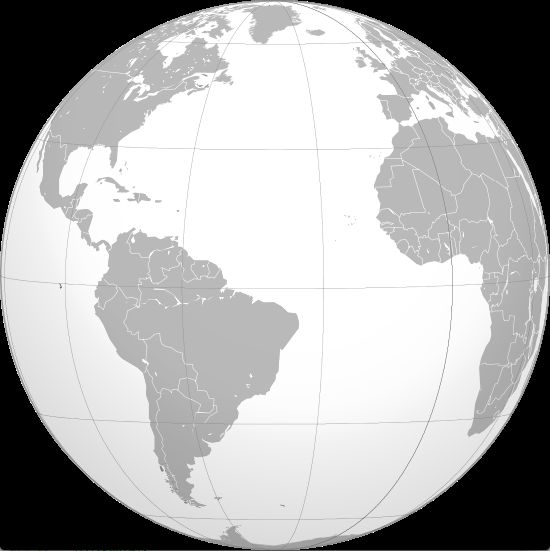
\includegraphics[scale = 0.2]{img/globe}
                \caption{Grayscale image}
        \end{subfigure}
		\quad
        \begin{subfigure}[b]{0.3\textwidth}
                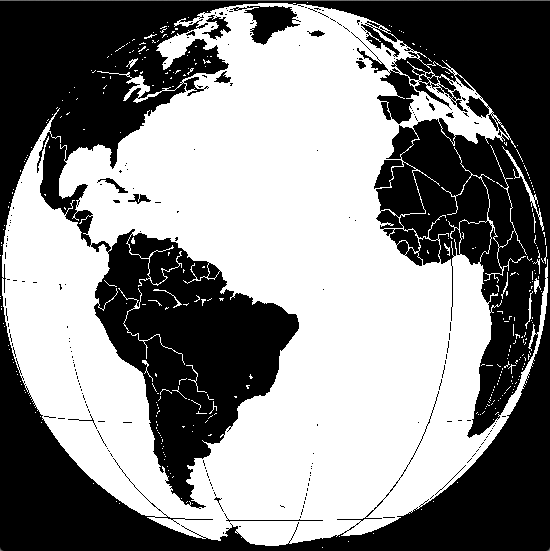
\includegraphics[scale = 0.2]{img/post_threshold}
                \caption{Thresholded image}
        \end{subfigure}
		\caption{An example of applying a threshold on a grayscale image. This example use the threshold value \textit{T} = 200}
		\label{fig:threshold_example}
\end{figure}

Now what happens if we you are interested in a color? To use standard thresholding we first need to convert \emph{src} to a grayscale image. However doing so might result in an image that have lost important information as can be seen in Figure \ref{fig:RGB2GRAY}. As shown, you have no way of differentiating the blue and green color.

\begin{figure}
        \centering
        \begin{subfigure}[b]{0.3\textwidth}
                
\includegraphics[scale=0.5]{img/RGB}
                \caption{RGB image}
        \end{subfigure}
		\quad
        \begin{subfigure}[b]{0.3\textwidth}
                
\includegraphics[scale=0.5]{img/GrayRGB}
                \caption{Grayscale image}
        \end{subfigure}
		\caption{Example of grayscaling a color image}
		\label{fig:RGB2GRAY}
\end{figure}

A step in the right direction would be to define the threshold value \textit{T} as a scalar consisting of three values - one for each color channel. We will denote this threshold scalar as \textit{S} and define it as shown in Equation \ref{eq:thresholdscalar}.

\begin{equation}
S =  
\begin{pmatrix}
  S_{R}\\
  S_{G}\\
  S_{B}\\
\end{pmatrix}
\label{eq:thresholdscalar}
\end{equation}

To apply it to an RGB image we need to change Equation \ref{eq:binarythresholding} to the one shown in Equation \ref{eq:threshold_RGB}.

\begin{equation}
{dst_i} = {src_i}_R \geq S_R \wedge {src_i}_G \geq S_G \wedge {src_i}_B \geq S_B? 255: 0
\label{eq:threshold_RGB}
\end{equation}

This makes it much easier to differentiate between colors. In Figure \ref{fig:RGB_Thresh} a threshold attempt using this method directly on the RGB image is shown.

\begin{figure}
        \centering
        \begin{subfigure}[b]{0.3\textwidth}
                
\includegraphics[scale=0.5]{img/RGB}
                \caption{RGB image}
        \end{subfigure}
		\quad
        \begin{subfigure}[b]{0.3\textwidth}
                
\includegraphics[scale=0.5]{img/RGBThresh}
                \caption{Thresholded image}
        \end{subfigure}
		\caption{Example of thresholding a color image with Equation \ref{eq:threshold_RGB} using the scalar \textit{S}=(0,100,0)}
		\label{fig:RGB_Thresh}
\end{figure}

However one issue remains - what if you want to find a color among similar colors? The problem is illustrated in Figure \ref{fig:green_fail} using the same scalar as in Figure \ref{fig:RGB_Thresh}.

\begin{figure}
        \centering
        \begin{subfigure}[b]{0.3\textwidth}
                
\includegraphics[scale=0.5]{img/green}
                \caption{RGB image}
        \end{subfigure}
		\quad
        \begin{subfigure}[b]{0.3\textwidth}
                
\includegraphics[scale=0.5]{img/simpleRGBThresh}
                \caption{Thresholded image}
        \end{subfigure}
		\caption{Example of thresholding a color image with Equation \ref{eq:threshold_RGB} using the scalar \textit{S}=(0,100,0). Unlike before the result is unsatisfactory.}
		\label{fig:green_fail}
\end{figure}

The solution is to specify a \textit{range} of acceptable values instead of just a threshold. We will specify two scalars; S Upper, \textit{SU}, and S Lower, \textit{SL}.

\begin{equation}
SL =  
\begin{pmatrix}
  SL_{R}\\
  SL_{G}\\
  SL_{B}\\
\end{pmatrix}
\label{eq:thresholdlower}
\end{equation}

\begin{equation}
SU =  
\begin{pmatrix}
  SU_{R}\\
  SU_{G}\\
  SU_{B}\\
\end{pmatrix}
\label{eq:thresholdupper}
\end{equation}

We will use the definitions in Equations \ref{eq:thresholdlower} and \ref{eq:thresholdupper} to update Equation \ref{eq:threshold_RGB}. The changes can be seen in Equation \ref{eq:threshold_range}.

\begin{equation}
{dst_i} = SU_R \geq {src_i}_R \geq SL_R \wedge SU_G \geq {src_i}_G \geq SL_G \wedge SU_B \geq {src_i}_B \geq SL_B? 255: 0
\label{eq:threshold_range}
\end{equation}

Using a range to specify a color instead will yield a much more satisfactory result as shown in Figure \ref{fig:green_final}. In summary, both grayscale thresholding, and color thresholding can be used to find ants of certain colors in an image.\\

\begin{figure}
        \centering
        \begin{subfigure}[b]{0.3\textwidth}
                
\includegraphics[scale=0.5]{img/green}
                \caption{RGB image}
        \end{subfigure}
		\quad
        \begin{subfigure}[b]{0.3\textwidth}
                
\includegraphics[scale=0.5]{img/finalthresh}
                \caption{Thresholded image}
        \end{subfigure}
		\caption{Example of thresholding a color image with Equation \ref{eq:threshold_range} using the range \textit{SL}=(0,100,0) and \textit{SU}=(1,150,10). We have sucessfully located the dark green color area.}
		\label{fig:green_final}
\end{figure}

\newpage

\noindent \textbf{Dilation and Erosion} \par
% Forklar at vi har en kernel, B, med størrelsen s, der bliver anvendt på hver pixel, p, i et billede A.
% Angiv at dilating finder local optima, og at eroding finder local minima.
% Angiv at de her metoder bliver brugt EFTER thresholding for at "rense" billedet. \\

When locating an ant, there might be many small bright dots that make the ant hard to see. This can be improved by using erosion or dilation, which are the basic concepts of \textit{morphological transformations} \cite{theory1}, depending on the image in question. These concepts are mostly used to remove noise, isolating individual elements or joining disparate elements in an image \cite{theory1}. Dilation and erosion are applied to either grayscale or binary images, and are often used to clean up after thresholding to make it easier to analyze.\\

The way both erosion and dilation are applied to an image is by defining a kernel, denoted \textit{B}, that will be applied to an image (or part of an image), denoted \textit{A}. The kernel can be any shape or size, however it is often a square where the sides are uneven, e.g. 3x3, 5x5, 7x7 and so on \cite{theory1}. A kernel has an \textit{anchorpoint}, which is the pixel in \emph{A} that erosion or dilation is applied to, and the result is stored in the corresponding point in the destination image, \textit{dst(i,j)}. Figure \ref{fig:kernel_ed} shows an example of a kernel and its anchorpoint in the center. \\

\begin{figure}[ht!]
  \centering
    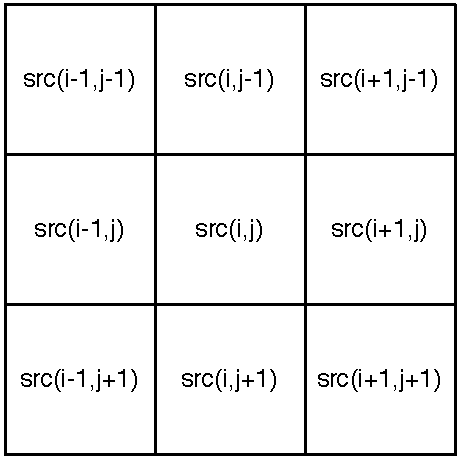
\includegraphics[scale=0.50]{img/Kernel_ED.pdf}
  \caption{Given a pixel, \emph{src(i,j)}, the kernel covers the neighbouring pixels. Shown here is a 3x3 kernel.}
  \label{fig:kernel_ed}
\end{figure}

When transforming an image using dilation, whenever the kernel is applied to a new anchorpoint, the \textit{local maximum} is used \cite{theory1}. When eroding an image the \textit{local minimum} is used \cite{theory1}. Naturally, compared to the original image, bright areas are expanded when dilating, and dark areas are expanded when eroding. However one cannot say that e.g. eroding removes noise and dilating does not. It depends on the image which the transformation is applied to. Figure \ref{fig:sample_kernel} shows an example of pixels used to determine the outcome of the anchorpoint in the destination image. \\

\begin{figure}[ht!]
  \centering
    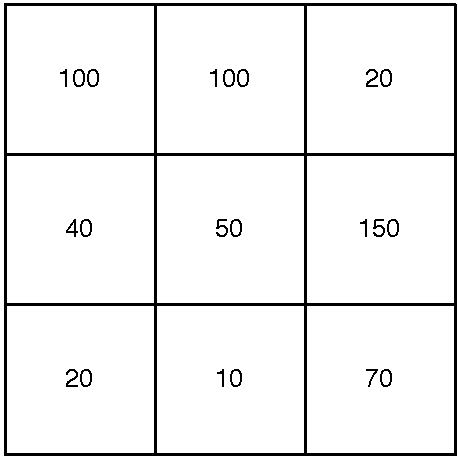
\includegraphics[scale=0.50]{img/sample_kernel.pdf}
  \caption{An example of a kernel within a source image, \emph{src}, with pixel values inserted. The value assigned to the destination image, \emph{dst(i,j)}, is 10 if erosion is chosen, or 150 if dilation is chosen.}
  \label{fig:sample_kernel}
\end{figure}

An example of how this applies to a real image is shown in Figure \ref{fig:erodedilate}. It is clear from this example how erosion and dilation affects an image.\\

\begin{figure}[!ht]
        \centering
        \begin{subfigure}[b]{0.3\textwidth}
                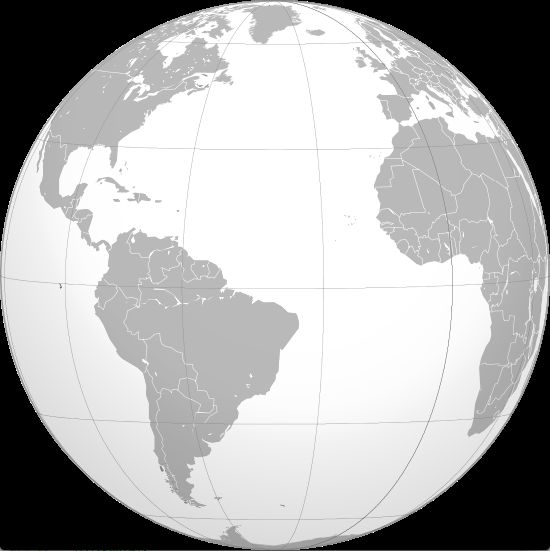
\includegraphics[scale = 0.2]{img/globe}
                \caption{Grayscale image}
        \end{subfigure}
		\quad
        \begin{subfigure}[b]{0.3\textwidth}
                
\includegraphics[scale = 0.2]{img/erode}
                \caption{Eroded image}
        \end{subfigure}
		\quad
        \begin{subfigure}[b]{0.3\textwidth}
                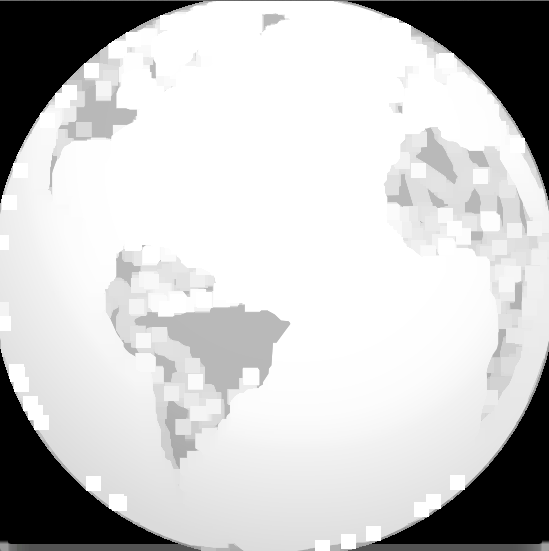
\includegraphics[scale = 0.2]{img/dilate}
                \caption{Dilated image}
        \end{subfigure}
		\caption{Eroding and dilating an image. Eroding expands dark areas and dilation expands bright areas. This example uses a 7x7 kernel.}
		\label{fig:erodedilate}
\end{figure}

Unlike thresholding we cannot apply erosion or dilation to RGB images due to the nature of RGB values. Imagine the clear colors, red (255,0,0), green (0,255,0) and blue(0,0,255) - in this case we cannot argue which color is \textit{greater} or \textit{smaller} than the other? We can with grayscale and binary images since we can safely say that the pixel value 150 is smaller than 255, and 0 is smaller than 1. In summary, we have presented techniques to make ants much clearer in an image with a lot of noise, that might prevent us from properly finding an ant.\\

\noindent \textbf{Contrast and Brightness} \par
Where dilation and erosion sought to expand either dark or bright areas, contrast and brightness seek to change the overall brightness or darkness of an image or the absolute difference between dark and bright pixels. This can make it easier to find an ant in an image where the image is either too bright, or too dark.\\

To increase the absolute difference between two pixels, or \textit{increasing the contrast of the image}, each pixel in an image is multiplied with the same scalar, denoted $\alpha$. Since images are matrices this method is equal to \textit{scalar multiplication} shown in Equation \ref{eq:matrix_mul}.

\begin{equation}
\alpha \times 
\setlength{\arraycolsep}{5pt}
 \begin{bmatrix}
  a & b & c \\
  d & e & f \\
  g & h & i \\
 \end{bmatrix} =
 \setlength{\arraycolsep}{5pt} 
 \begin{bmatrix}
  \alpha \times a & \alpha \times b & \alpha \times c \\
  \alpha \times d & \alpha \times e & \alpha \times f \\
  \alpha \times g & \alpha \times h & \alpha \times i \\
 \end{bmatrix}
 \label{eq:matrix_mul}
\end{equation}

To increase the brightness, a scalar is added to each pixel, denoted $\beta$. This way the absolute difference between each pixel is kept, however all pixels get darker or brighter depending on the scalar. Similar to contrast this operation is equal to \textit{scalar addition} as shown in Equation \ref{eq:matrix_add}. To make the pixels brighter a positive scalar is added, to make it darker a negative scalar is added. Figure \ref{fig:bright_contrast} shows the result of contrasting and increasing the brightness of an image. Contrast and brightness are used to make dark, bright and diffuse images easier to analyse. In summary, contrast and brightness can help improve the image quality, making it much easier to find an ant, or distinguish it from other parts of the image.\\

\begin{equation}
\beta + 
\setlength{\arraycolsep}{5pt}
 \begin{bmatrix}
  a & b & c \\
  d & e & f \\
  g & h & i \\
 \end{bmatrix} =
 \setlength{\arraycolsep}{5pt} 
 \begin{bmatrix}
  \beta + a & \beta + b & \beta + c \\
  \beta + d & \beta + e & \beta + f \\
  \beta + g & \beta + h & \beta + i \\
 \end{bmatrix}
 \label{eq:matrix_add}
\end{equation}

\begin{figure}
        \centering
        \begin{subfigure}[b]{0.3\textwidth}
                
\includegraphics[scale = 0.2]{img/colorGlobe}
                \caption{Source image}
        \end{subfigure}
		\quad
        \begin{subfigure}[b]{0.3\textwidth}
                
\includegraphics[scale = 0.2]{img/globeBright}
                \caption{Brightened image}
        \end{subfigure}
        \begin{subfigure}[b]{0.3\textwidth}
                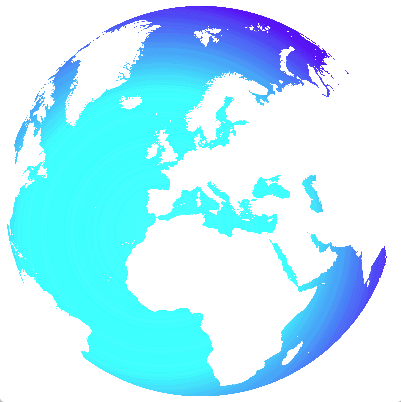
\includegraphics[scale = 0.2]{img/globeContrast}
                \caption{Contrasted image}
        \end{subfigure}
		\caption{Example of increasing the contrast and brigtness of an image. For this example $\alpha = 5$ and $\beta = 100$}
		\label{fig:bright_contrast}
\end{figure}

\noindent \textbf{Image Segmentation} \par
Image segmentation is the process of partitioning all the pixels in an image into \textit{S} segments (or superpixels). The goal is to simplify or change the representation of an image such that it is easier to analyze. It is mostly used to locate objects that consist of a range of similar colors, that is combined into a single colored object after segmentation, thus making it easier to find \cite{theory1}. Image segmentation is therefore the process of assigning a label to a pixel, such that pixels with the same label share certain visual characteristics. The result of image segmentation is a set of segments that covers the entire image. Thresholding, as described earlier, is the simplest method of segmenting an image. This can be an important technique in finding the ant, should thresholding alone not be enough.\\

One of the most common algorithms to segment images is the \textit{k-means} algorithm \cite{theory2}. K-means is a \textit{clustering algorithm} often used in \textit{datamining}. K-means takes a set of unclassified data, and classifies it. It does so by assigning all the data to \textit{K} different clusters, and iteratively assign each element to the cluster it is most similar to after new \textit{centroids} have been assigned or created. The algorithm terminates when data no longer changes clusters or a predefined number of iterations have completed. Even though more robust classification algorithms exists, \textit{k-means} is often used simply because each iteration is relatively fast. The algorithm works as follows:

\begin{enumerate}
  \item Randomly select \textit{k} objects in the dataset \textit{D}, which initially represents the centroid for each cluster.
  \item Each object in \textit{D}, is then assigned to the centroid it is most similar to.
  \item For each cluster, it computes a new centroid from the previously assigned object and repeats step 2.
  \item If all clusters are unchanged between two iterations, the algorithm terminates.
\end{enumerate}

An example of using k-means to cluster an image is shown in Figure \ref{fig:segmentation}. In summary, image segmentation provides a powerful way to easily simplify an image, which can make ant detection easier.\\

\begin{figure}
        \centering
        \begin{subfigure}[b]{0.3\textwidth}
                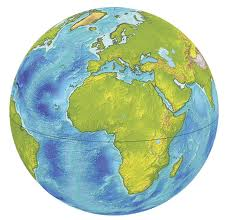
\includegraphics[scale = 0.5]{img/earth}
                \caption{Source image}
        \end{subfigure}
		\quad
        \begin{subfigure}[b]{0.3\textwidth}
                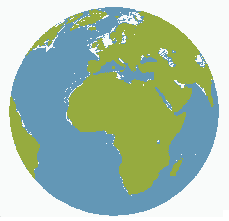
\includegraphics[scale = 0.5]{img/earth_segment}
                \caption{Segmented image}
        \end{subfigure}
		\caption{Example of segmenting an image. In this example the number of clusters specified is 3.}
		\label{fig:segmentation}
\end{figure}

\noindent \textbf{Background subtraction} \par
Background substraction (also known as foreground detection) is a process often used to detect moving objects with a static camera \cite{theory1}. The idea is that the background remains roughly the same in every image in a video stream, while moving objects enter and leave the stream shortly after, or become part of the background after some time have passed. The rationale is to have a background image (or reference point) and then substract the image with the new object in it. This technique can be useful for tracking a moving ant, assuming the background remains roughly the same in the test setup. Computing the difference between the foreground and background will result in an image with only the moving object in it, that can be used for analysis. The absolute difference is computed almost like a standard \textit{matrix substraction} as shown in Equation \ref{eq:matrix_sub}. An example of background subtraction is shown in Figure \ref{fig:background_filtering}.\\

\begin{equation}
\setlength{\arraycolsep}{5pt}
 \begin{bmatrix}
  a & b \\
  c & d \\
 \end{bmatrix} - 
 \setlength{\arraycolsep}{5pt} 
 \begin{bmatrix}
  e & f \\
  g & h \\
 \end{bmatrix} =
 \setlength{\arraycolsep}{5pt} 
 \begin{bmatrix}
  abs(a-e) & abs(b-f) \\
  abs(c-g) & abs(d-h) \\
 \end{bmatrix}
 \label{eq:matrix_sub}
\end{equation}

\begin{figure}
        \centering
        \begin{subfigure}[b]{0.3\textwidth}
                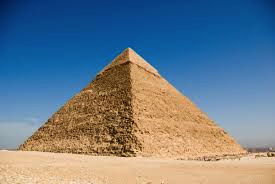
\includegraphics[scale = 0.35]{img/pyramid}
                \caption{Background image}
        \end{subfigure}
		\quad
        \begin{subfigure}[b]{0.3\textwidth}
                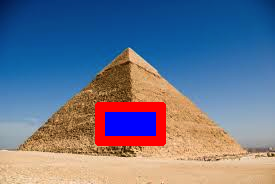
\includegraphics[scale = 0.35]{img/pyramid_new}
                \caption{Foreground image}
        \end{subfigure}
        \begin{subfigure}[b]{0.3\textwidth}
                
\includegraphics[scale = 0.35]{img/pyramid_object}
                \caption{Object detection}
        \end{subfigure}
		\caption{Example of detecting a new object on a static background. In this example all differences greater than zero is set to 255.}
		\label{fig:background_filtering}
\end{figure}

\subsubsection{Computer Vision Framework} \mbox{}\par
\label{framework}
The theory behind computer vision techniques is solid. However to track an ant in an image, theory and implementation is not enough. We have to keep in mind that we must locate the ant in several consecutive images, without delaying the entire process, allowing the ant to escape the camera. Therefore efficiency is a key aspect as well. Choosing an efficient framework to help us track ants is therefore of utmost importance. OpenCV is such a framework.\\

OpenCV is short for Open Computer Vision, and is an open source project started in 1999 and since maintained by Intel. It is written in C and C++ and runs on Linux, Windows and Mac OS X. OpenCV was designed from the beginning to be computationally efficient with a strong focus on real-time applications. Another goal is to provide a simple-to-use computer vision infrastructure. Since its initial creation, OpenCV has matured gradually, and along with it computer vision as well. Today, OpenCV and computer vision is used in a broad context from web applications to surveillance and aerial street maps.\\

Other computer vision frameworks exist but are limited on several parameters. As stated in the requirements, tracking had to be done in C/C++ which rules out frameworks for higher level languages such as PyCVF for Python, imageJ for Java and OpenClooVision for C\#. Furthermore several frameworks exist that extends OpenCV or creates a simpler abstraction layer such as SimpleCV and other frameworks offers a very limited amount of features such as VisionBlocks. As a result OpenCV was chosen to be the framework of choice, both because of maturity and effeciency, but also because of the amount of computer vision features offered to its users.

\subsubsection{Realization} \mbox{}\par
Having presented several computer vision techniques and the framework used, this section will focus on applying these techniques in a real world scenario to find an ant within an image from a webcam. To be able to track the ant of interest and make it distinguishable from other ants, we will paint it with a color that is easier to detect than the ant itself. We want to track the ants on real dirt, and not just a opaque background, and the ant available are either dark brown or black (as seen in image \emph{a} in Figure \ref{fig:antcoloring}) closely resembling dirt in their native environment. It is therefore important to choose a color that is easy to detect on such material. For this reason we have chosen white paint.\\

The image in Figure \ref{fig:ant} will be used as a reference point when showing how a certain computer vision technique performs in locating the ant.

\begin{figure}[ht!]
  \centering
    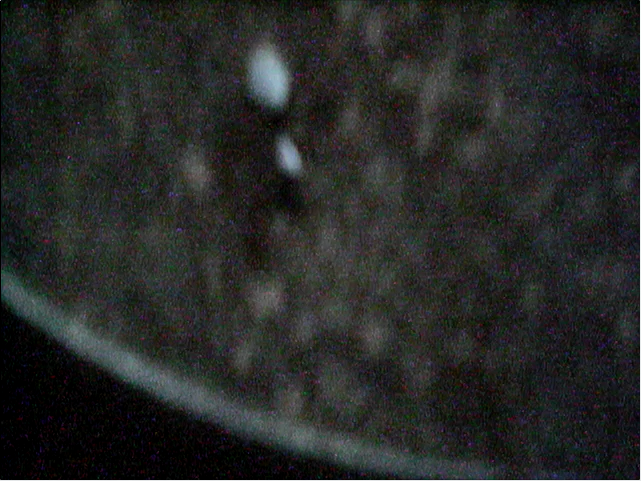
\includegraphics[scale=0.25]{img/ant.png}
  \caption{Unprocessed image of an ant.}
  \label{fig:ant}
\end{figure}

It is evident from the image in Figure \ref{fig:ant}, that the overall image is very dark. The ant itself is very hard to see, and even the white areas are dark. A way to improve this is to use the theory of \emph{Contrast and Brightness}(Found in Section \ref{sec:tracking_theory}) to improve the lighting condition of the image. Figure \ref{fig:contrast_ant} shows the result of applying contrast or brightness to Figure \ref{fig:ant}. \\

\begin{figure}
        \centering
        \begin{subfigure}[b]{0.4\textwidth}
                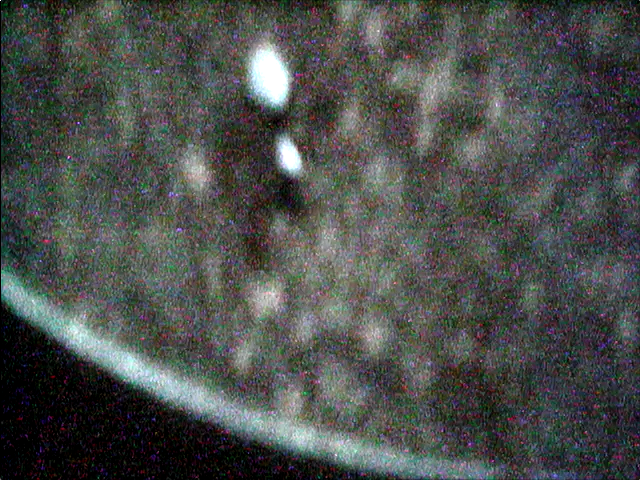
\includegraphics[scale = 0.2]{img/contrast2times}
                \caption{$\alpha = 2$}
        \end{subfigure}
		\quad
        \begin{subfigure}[b]{0.4\textwidth}
                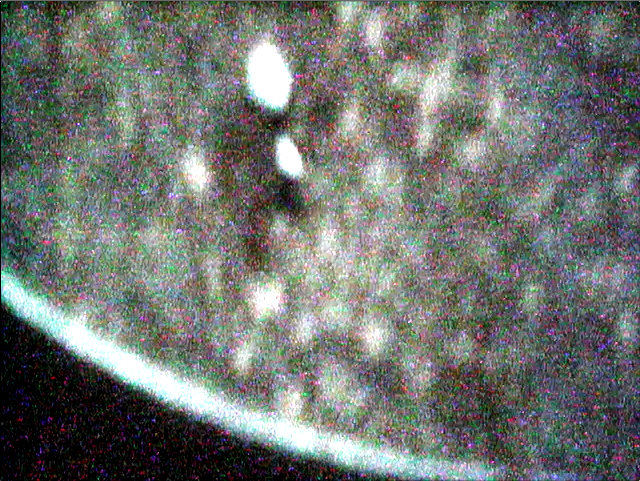
\includegraphics[scale = 0.2]{img/contrast3times}
                \caption{$\alpha = 3$}
        \end{subfigure} \hfill \\ \mbox{}\\
        \begin{subfigure}[b]{0.4\textwidth}
                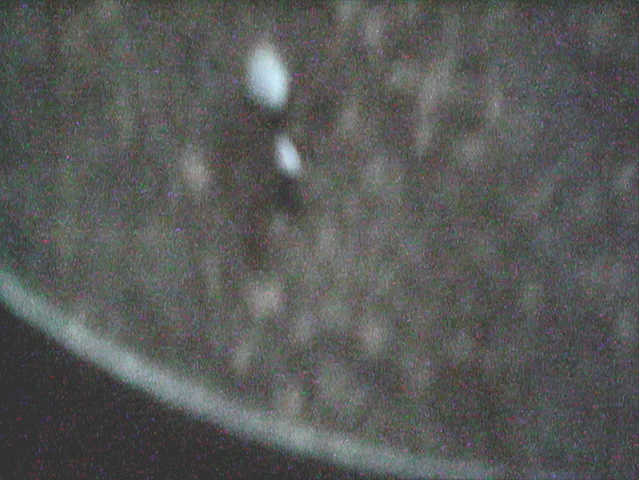
\includegraphics[scale = 0.2]{img/bright50}
                \caption{$\beta = 50$}
        \end{subfigure}
		\quad
        \begin{subfigure}[b]{0.4\textwidth}
                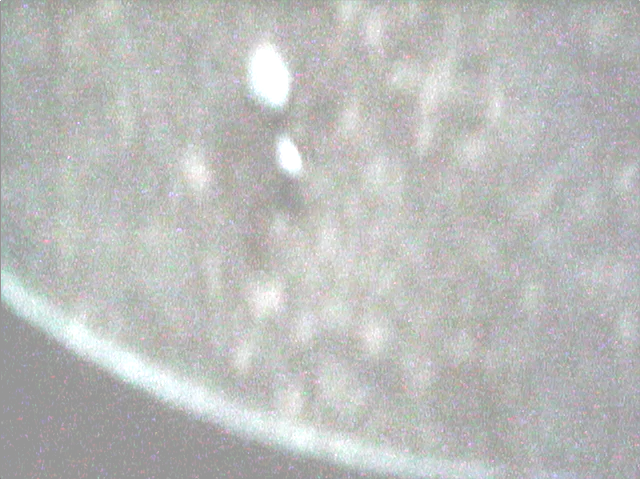
\includegraphics[scale = 0.2]{img/bright150}
                \caption{$\beta = 150$}
        \end{subfigure}
		\caption{Applying brightness(\emph{c} and \emph{d}) or contrast(\emph{a} and \emph{b}) to the ant image.}
		\label{fig:contrast_ant}
\end{figure}

It is clear from Figure \ref{fig:contrast_ant} that image \emph{c} and \emph{d} does not provide the best result. Even though the image is indeed brightened, differentiating between the ant and the background has not become much easier. Whether image \emph{a} or \emph{b} provides the best result comes down to what we want the most - that the object we look for is as close to clear white as possible, or that it is the most distinguishable object in the image. In general, it is better for colors to be distinguishable than trying to make them match a specific color intensity. The result of image \emph{a} is therefore preferable. \\

Now that we have improved the overall quality of the image, the next task is to isolate the ant in the improved image. For this task we have three techniques available; \emph{thresholding}, \emph{image segmentation} and \emph{background subtraction}. Background subtraction requires that the background in any two compared frames are close to equal. Since the mobile camera is moving during tracking, this technique is not optimal. This leaves us with image segmentation and thresholding.\\

Figure \ref{fig:segment_ant} shows examples of running image segmentation with different numbers of segments, \textit{K}, defined on image \emph{a} from Figure \ref{fig:contrast_ant}. It is clear from these tests that a certain number of segments are neccessary to give a satisfactory result. $K=8$ and $K=10$ clearly gives the best results, however it comes at a cost; segmenting these images simply takes too much time for the camera to keep up with the ant. Even with only one segmentation attemp for each image, it takes around one second or more to produce a result. Considering this needs to be done \emph{multiple} times within a second when using a live camera feed, this solution is simply not feasible or possible for tracking. An ant can easily move out of a frame, simply because it is too slow or the ant is too fast.\\

\begin{figure}
        \centering
        \begin{subfigure}[b]{0.4\textwidth}
                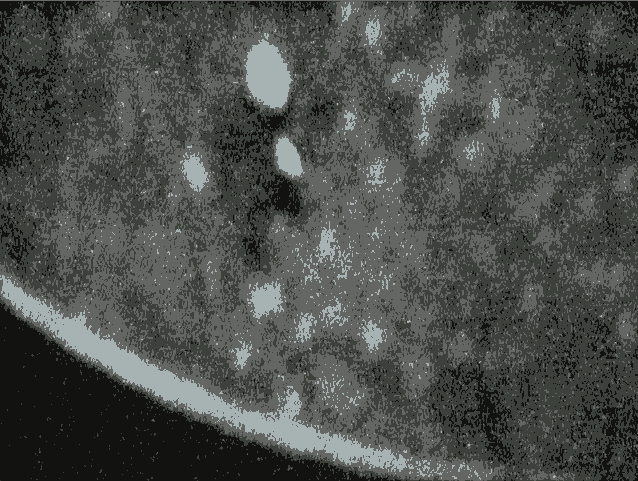
\includegraphics[scale = 0.2]{img/segment4}
                \caption{K = 4}
        \end{subfigure}
		\quad
        \begin{subfigure}[b]{0.4\textwidth}
                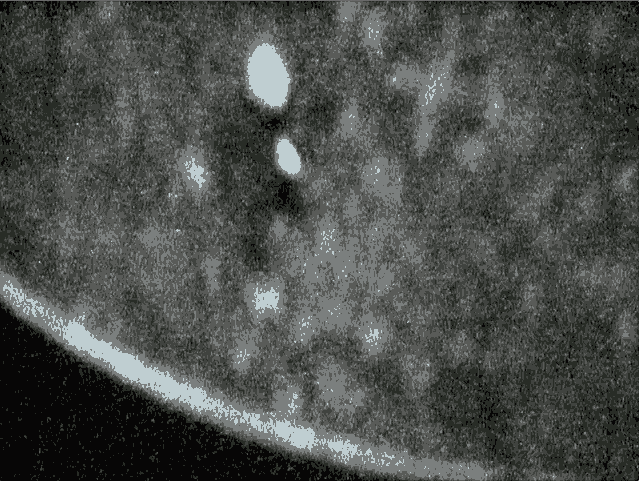
\includegraphics[scale = 0.2]{img/segment6}
                \caption{K = 6}
        \end{subfigure} \hfill \\ \mbox{}\\
        \begin{subfigure}[b]{0.4\textwidth}
                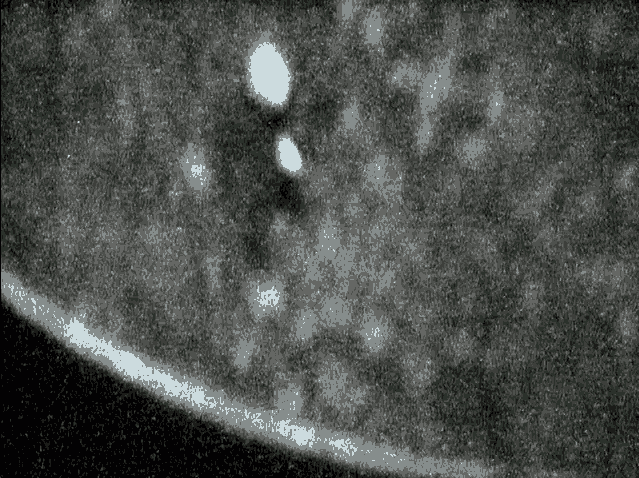
\includegraphics[scale = 0.2]{img/segment8}
                \caption{K = 8}
        \end{subfigure}
		\quad
        \begin{subfigure}[b]{0.4\textwidth}
                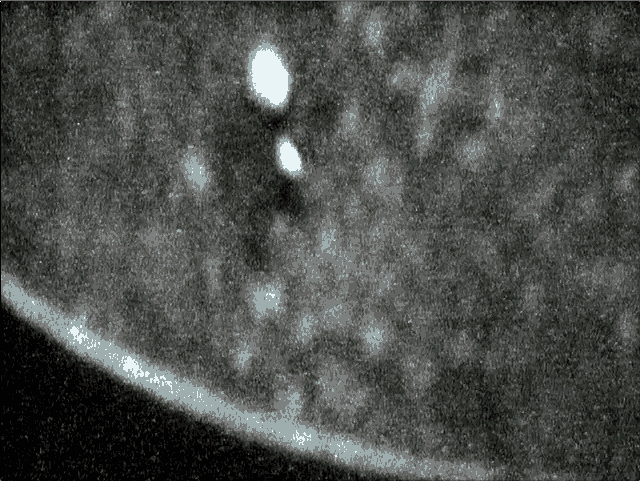
\includegraphics[scale = 0.2]{img/segment10}
                \caption{K = 10}
        \end{subfigure}
		\caption{Segmenting the ant image.}
		\label{fig:segment_ant}
\end{figure}

This leave us with only one option; thresholding. Figure \ref{fig:threshant} shows thresholding attemps on a grayscale version of image \emph{a} from Figure \ref{fig:contrast_ant}. The results of different thresholds shows two things; firstly that image \emph{d} is a good threshold result and secondly that we need a rather high threshold value to get it. In contrast to segmentation, applying a threshold to our image is much faster and is usable with a mobile camera.\\

\begin{figure}
    \vspace{-2em}
        \centering
        \begin{subfigure}[b]{0.4\textwidth}
                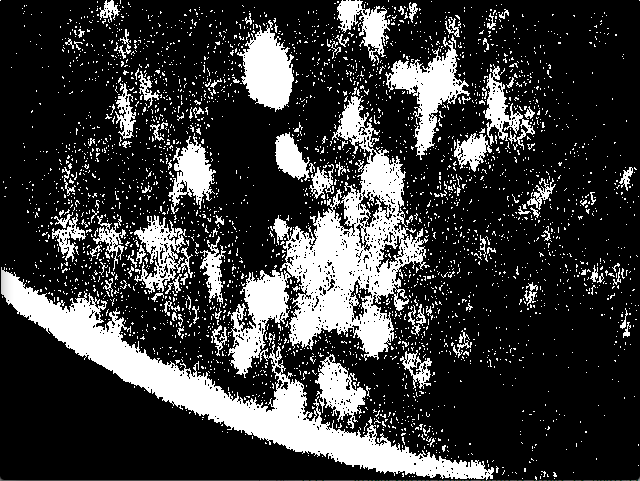
\includegraphics[scale = 0.2]{img/thresh100}
                \caption{T = 100}
        \end{subfigure}
		\quad
        \begin{subfigure}[b]{0.4\textwidth}
                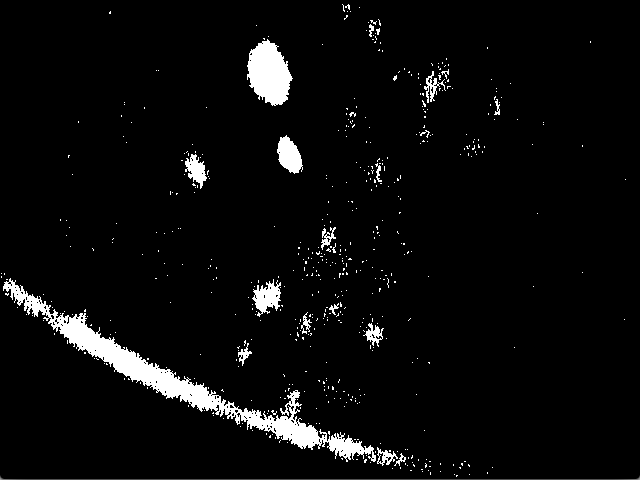
\includegraphics[scale = 0.2]{img/thresh150}
                \caption{T = 150}
        \end{subfigure} \hfill \\ \mbox{}\\
        \begin{subfigure}[b]{0.4\textwidth}
                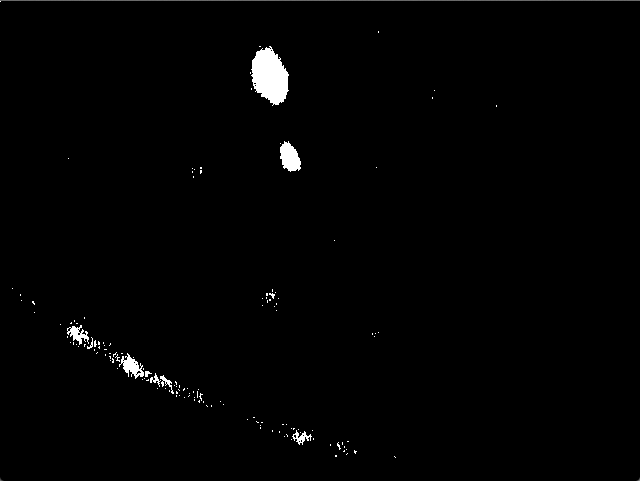
\includegraphics[scale = 0.2]{img/thresh200}
                \caption{T = 200}
        \end{subfigure}
		\quad
        \begin{subfigure}[b]{0.4\textwidth}
                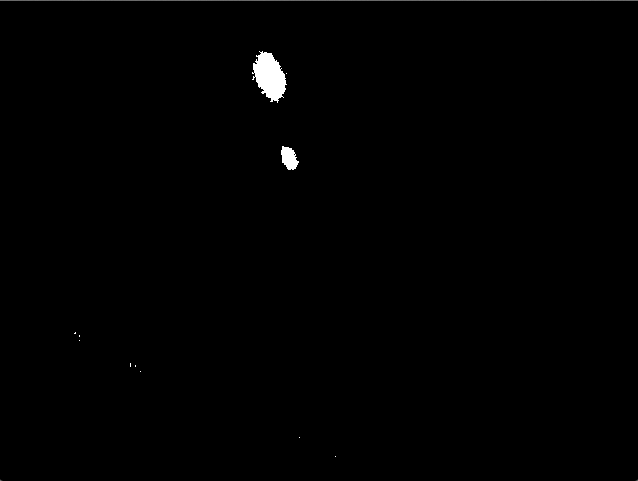
\includegraphics[scale = 0.2]{img/thresh240}
                \caption{T = 240}
        \end{subfigure}
		\caption{Thresholding the ant image.}
		\label{fig:threshant}
        \vspace{-2em}
\end{figure}

Now that we have a satisfactory binary image that clearly shows the position of the ant, the next step is to actually get the position of the ant within the image. For this purpose we use \textit{blob detection}. In short, blob detection is a computer vision technique encapsulating mathematical methods that are aimed at detecting regions in a digital image. These regions can differ in properties such as brightness and color from the regions surrounding it. Where segmentation seeks to partition an image, blob detection seek to extract the partitions. All the pixels in a blob are considered to share similar properties. \\

The binary image \emph{d} from Figure \ref{fig:threshant} clearly shows that we have two blobs available, that are rather large. This is of course ideal, but we might also have cases where we have smaller blobs caused by reflections of the dirt or water. Therefore it is not enough to extract all blobs from the image and use the first one - we should always use the largest blob available in the image, which hopefully, is our ant. The result of finding the largest blob in our binary image is shown in Figure \ref{fig:finalResult}.

\begin{figure}
    \captionsetup{justification=centering}
        \centering
        \begin{subfigure}[b]{0.45\textwidth}
                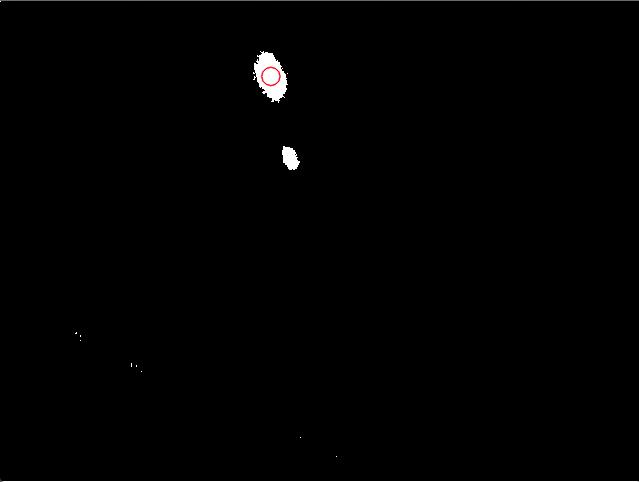
\includegraphics[scale = 0.25]{img/threshblob}
                \caption{\mbox{}\\Detected blob drawn on binary image}
        \end{subfigure}
		\quad
        \centering
        \begin{subfigure}[b]{0.45\textwidth}
                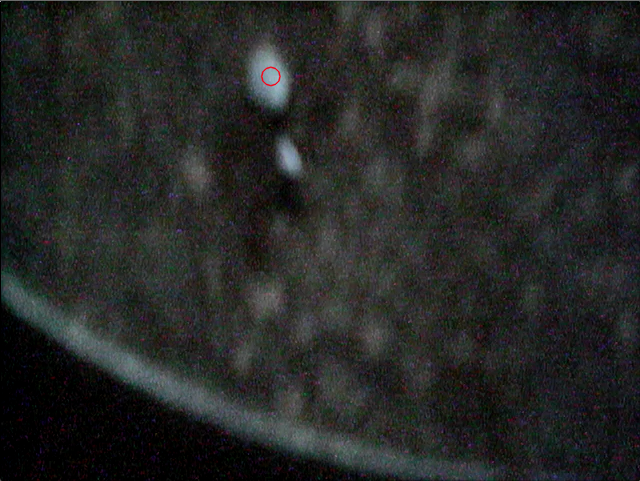
\includegraphics[scale = 0.25]{img/srcblob}
                \caption{\mbox{}\\Detected blob drawn on original image}
        \end{subfigure}
		\caption{Final result of finding the ant in our image. The detected blob is found on both the thresholded image and the original ant image.}
		\label{fig:finalResult}
        \vspace{-2em}
\end{figure}

Concluding this chapter we summarize the process of going from a raw image input to a successfully detected ant, based on both the choices and experiments from this chapter. The process is as follows:

\begin{enumerate}
    \item Increase the contrast of the raw image with an $\alpha$ value of at least 2.0.
    \item Convert the contrasted image to grayscale.
    \item Threshold the grayscale image with a threshold value of at least 240.
    \item Run blob detection on the thresholded image.
    \item Output the largest blob from the blob detection on the original image.
\end{enumerate}

\subsubsection{Optimizing the Realized Solution on Windows} \mbox{}\par
\label{sec:optimizing}
During development we observed strange behavior with the OpenCV implementation. On OS X processing a single image took between 28 and 32 ms, however the same code performed much worse on our Windows test machine. This is strange considering that the computer running OS X has much older and much slower hardware than the Windows machine. In comparison, processing the same image on Windows, with the same implementation took between 200 and 300 ms and sometimes close to 500 ms for a single image. We ran several tests to find out why, and even when comparing the OpenCV installations we found no difference in what features were enabled and disabled. We also tested the implementation on another Windows machine with more powerful hardware, but the behavior was the same. To solve the problem we tried two things:\\

\begin{enumerate}
    \item Compile the OpenCV source using CMake \cite{cmake}, instead of using the precompiled binaries available at the OpenCV download page.
    \item Use the OpenCV CUDA \cite{cuda} Graphical Processing Unit (GPU) module that can be used to optimize image processing on computers with NVidia GPU's.
\end{enumerate}

After compiling the OpenCV source code on the machine where it should be used, we found no difference in performance at all. We therefore changed the implementation to use the enabled GPU module and moved some of the processing to the GPU. This greatly improved the performance. Processing time went down to a stable 27-30 ms on our test machine, allowing us to do processing in real time. We cannot say why Windows performs differently than OS X, however this is a satisfactory solution to the problem.\\

In conclusion we were able to use OpenCV to locate an ant in a frame using thresholding, contrasting and blob detection. The processing time of this were optimized using the OpenCV CUDA GPU module and enabled us to use this method in realtime when tracking an ant. 